\onecolumn
\subsection{Semesterticket}
Euer Studentenausweis berechtigt euch zur Fahrt auf vielen Zugstrecken in
Niedersachsen. Aktuelle Informationen zum Semesterticket gibt es auf den Seiten
des AStA (\nurl{http://www.asta.tu-bs.de/semesterticket.html}).
Es d"urfen nur Regionalexpress (RE) und Regionalbahn (RB) in der zweiten Klasse
benutzt werden.\\
Die folgenden Strecken d"urfen benutzt werden (ohne Gew"ahr):
\begin{table}[h]
\centering
\begin{tabular}{l|l|l|l}
	& & & \textbf{Nr. der}\\
	\textbf{von} & \textbf{"uber} & \textbf{bis} & \textbf{Kursbuchstrecke(n)}\\
	\hline
	Norddeich        &                      & Rheine (Westf)     & 395,390\\
	Emden            &                      & Emden Au"senhafen  & 396\\
	Weener           &                      & Leer (Ostfr)       & 397\\
	Leer (Ostfr)     & Bremen               & Hannover           & 390/380\\
	Nordenham        &                      & Bremen Hbf         & 391\\
	Salzbergen       & Osnabr"uck           & Hannover Hbf       & 375,370\\
	Osnabr"uck       & Bremen               & Hamburg Hbf        & 385/120\\
	Minden (Westf)   & Nienburg (Weser)     & Rotenburg (W)      & 124\\
	Hamburg-Harburg  & Cuxhaven             & Bremen Hbf         & 121/125\\
	Buchholz         & Soltau               & Hannover Hbf       & 123\\
	Bremen Hbf       & Soltau               & Uelzen             & 116\\
	Bremen Hbf       &                      & Bremen-Vegesack    & 126\\
	Uelzen           &                      & Schnega            & 305\\
	Uelzen           & Gifhorn              & Braunschweig       & 115\\
	Haste            & Weetzen              & Hannover Hbf       & 363\\
	Bad Pyrmont      & Hannover             & Hannover Flughafen & 363\\
	Löhne (Westf)    & Hannover             & Helmstedt          & 370/310\\
	Lehrte           &                      & Wolfsburg          & 300\\
	Hamburg Hbf      & Hannover             & G"ottingen         & 110/350\\
	Echem            &                      & L"uneburg          & 145\\
	L"uneburg        &                      & Dannenberg Ost     & 112\\
	Celle            & Lehrte               & Hildesheim Hbf     & 363/323\\
	Hannover Hbf     & Emmerke              & Goslar             & 320\\
	Braunschweig Hbf &                      & Wolfsburg          & 301\\
	Braunschweig Hbf & Sz-Ringelheim        & Holzminden         & 355\\
	Braunschweig Hbf & Bad Harzburg         & Kreiensen          & 353,354\\
	Braunschweig Hbf &                      & Sz-Lebenstedt      & 352\\
	Braunschweig Hbf & Wolfenb"uttel/Jerxhm & Helmstedt          & 312\\
	Braunschweig Hbf &                      & Hildesheim         & 313\\
	Braunschweig Hbf & Seesen               & Herzberg           & 358,355\\
	Ottbergen        & Northeim             & Walkenried         & 356/357\\
	Ottbergen        &                      & G"ottingen         & 356\\
	Bodenburg        & Hildesheim, Elze,    & B"unde (Westf)     & 321,322,372\\
	                 & Hameln               &                    & \\
	Helmstedt        & Magdeburg            & Halle              & 310/340\\
	Walkenried       &                      & Nordhausen         & 357\\
\end{tabular}
\end{table}

\clearpage
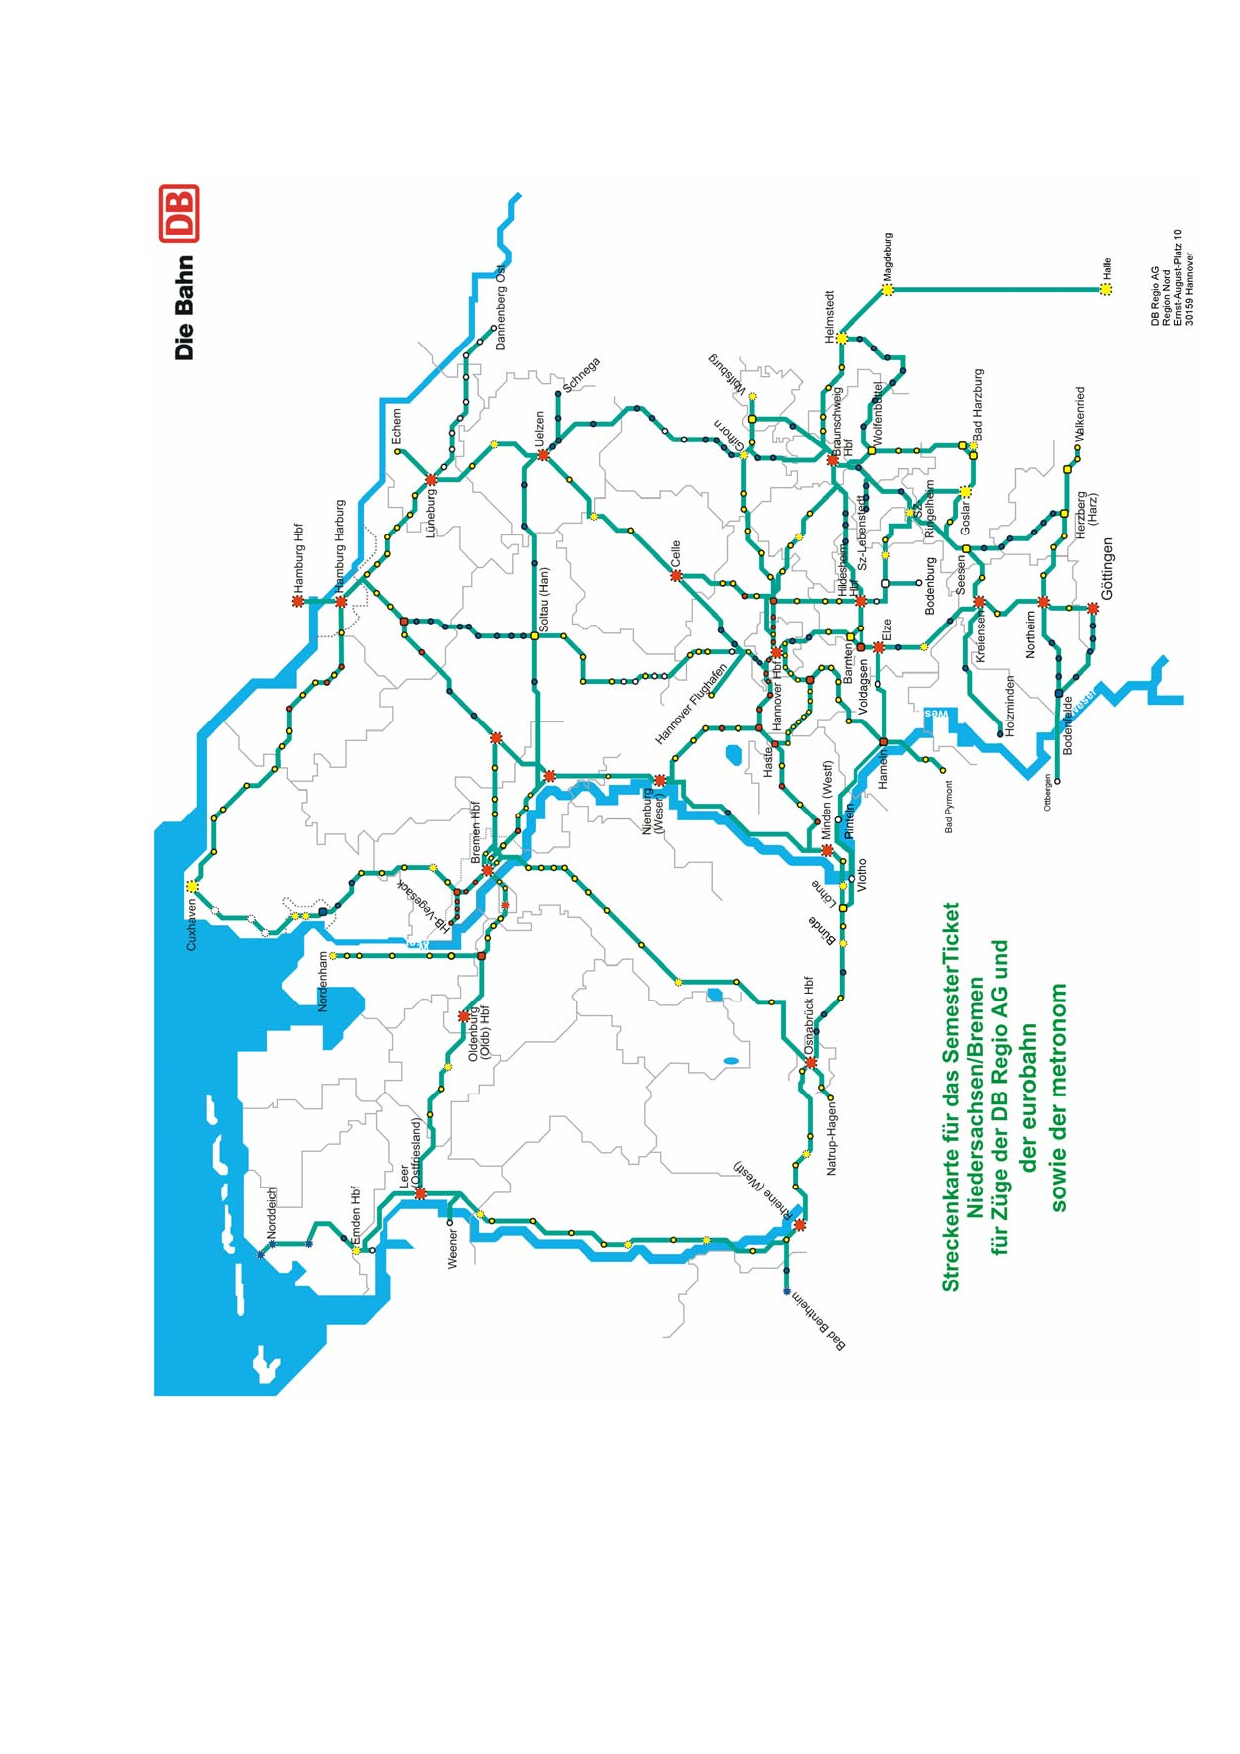
\includepdf{texte/nuetzliches/Beiblatt_10_06-09_07_Seite_2.pdf}